\documentclass{pramana}

\usepackage{graphicx,amsmath,bm}
%\usepackage[font=small]{caption}
\usepackage{subcaption}
\usepackage{hyperref}
\usepackage{lastpage}
\usepackage{multirow}
\usepackage{enumerate}

\usepackage{lipsum}

\captionsetup{font=normalsize,labelfont={bf,sf}}
\captionsetup[sub]{font=small,labelfont={bf,sf}}

%\newcommand{\papertitle}{Multi-Satellite Spectral Analysis of the Supersoft X-ray Source RX J0925.7-4758}
%\newcommand{\papertitle}{Multi-Observatory Spectral Analysis of the Supersoft X-ray Source RX J0925.7-4758}
\newcommand{\papertitle}{Multi-Observatory Spectral Analysis of the Supersoft X-ray Continuum of RX J0925.7-4758}
\newcommand{\authorone}{Parag Bhattacharya}
\newcommand{\authoroneaffiliation}{Department of Physics, Rangapara College, Rangapara, Assam - 784 505, India}
\newcommand{\authoremail}{bhattacharya.parag@gmail.com}
\newcommand{\authortwo}{Rabindra Mahato}
\newcommand{\authortwoaffiliation}{Department of Physics, Science College Kokrajhar, Kokrajhar, Assam - 783 370, India}
\newcommand{\authorthree}{Ranjeev Misra}
\newcommand{\authorthreeaffiliation}{Inter-University Centre for Astronomy and Astrophysics, Pune, Maharashtra - 411 007, India}
\newcommand{\authorfour}{Monmoyuri Baruah}
\newcommand{\authorfouraffiliation}{Department of Physics, Assam Don Bosco University, Tapesia, Assam - 782 402, India}


\title{\papertitle}
        
\author{\authorone\textsuperscript{1,4,*}, \authortwo\textsuperscript{2,4}, \authorthree\textsuperscript{3}\and \authorfour\textsuperscript{4}}
\affilOne{\textsuperscript{1} \authoroneaffiliation\\}
\affilTwo{\textsuperscript{2} \authortwoaffiliation\\}
\affilThree{\textsuperscript{3} \authorthreeaffiliation\\}
\affilFour{\textsuperscript{4} \authorfouraffiliation}

\newcommand{\source}{RX J0925.7-4758}

\renewcommand{\arraystretch}{1.8}


\begin{document}
    
    \twocolumn[{    
        \maketitle    
        \corres{\authoremail}
        
        %% Manuscript information: received, revised and accepted dates
        \msinfo{1 January 2015}{1 January 2015}{1 January 2015}
        
        %% Abstract
        \begin{abstract}
    The current work presents a comprehensive study on the spectral characteristics and parameters of the supersoft X-ray source \source. We utilize a dataset comprising six observations conducted by four different satellite missions spanning a time period of 25 years. Our objective is to identify a robust NLTE spectral model that can provide an acceptable fit to the continuum spectrum of \source, thereby enhancing our understanding of its astrophysical nature. The study employs rigorous spectral modeling and comparative analysis to establish a framework for characterizing the continuum spectrum of \source. The document also discusses the analysis of the supersoft spectrum of \source, including the challenges in reproducing its spectra using NLTE model atmospheres. The best-fit model consists of a pure hydrogen NLTE model with effective gravity of 7, multiplied with photoelectric absorption, ISM absorption and edge components. The effective temperature is found to be approximately of the order of $\sim$100 kK for all six observations, suggesting the presence of a hot accretion disk surrounding the white dwarf, which accretes matter from a companion main-sequence star. The study also analyzes the relative strengths of absorption edges in the spectrum and notes inconsistencies in the NICER observations. It makes a case for the need to explore and develop methods that study the latest high-resolution grating spectra, so as to obtain a more nuanced view of the astrophysics involving \source.
\end{abstract}

\keywords{X-rays: binaries, X-rays: individual: \source, methods: observational, techniques: spectroscopic}
% https://www.inaoep.mx/~ydm/aj_keywords.html

        
        %% PACS numbers
        \pacs{12.60.Jv; 12.10.Dm; 98.80.Cq; 11.30.Hv}    
    }]
    
    \doinum{12.3456/s78910-011-012-3}   % DOI number
    \artcitid{\#\#\#\#}                 % Article citation ID
    \volnum{123}                        % Volume number
    \year{2016}                         % Year of publication
    \pgrange{23--25}                    % Page range
    \setcounter{page}{23}               % Starting page
    \lp{25}                             % Last page

    %% Sections
    \section{Introduction}
    %To include the following
    %\begin{itemize}
        %\item Current literature on SSS
        %\item Current literature specifically on MR Vel -- focus on the lack of proper spectral analysis till date
        %\item Novelty of our approach -- elaborate on the reason for choosing multi-satellite data
        %\item Elaborate on the objective and what has been obtained in our work
    %\end{itemize}
    
    % Modified following reviewer comments 1.1 and 1.2:
    Supersoft X-ray sources (hereafter SSS) represent an important class of celestial objects. They were initially noticed in the soft X-ray survey  of the Large Magellanic Cloud galaxy (LMC) using the \textit{Einstein Observatory} by Long \textit{et al.} (1981) \cite{long81}. These objects were later recognized as a distinct class of intrinsically luminous X-ray sources by Trümper \textit{et al.} (1991) \cite{trumper1991x}, and also Greiner \textit{et al.} (1991) \cite{greiner1991rosat}, following the observation of more SSS in the LMC using the \textit{Roentgen Observatory Satellite} (\textit{ROSAT}). Subsequently, Kahabka and van den Heuvel (1997) \cite{kahabka97} have tabulated other SSS identified using \textit{ROSAT} in the Milky Way galaxy (hereafter Galactic SSS), the Small Magellanic Cloud galaxy (SMC), the Andromeda galaxy (M31) and the Local Group galaxy (NGC 55), in addition to those detected in the LMC. Ever since, hundreds of objects exhibiting similar characteristics have been documented, many of which are considered candidates or confirmed members of this class, thereby significantly expanding the catalogue of SSS \cite{kahabkatrumper1996, steinerdiaz1998, greiner2000, pietsch2003deep, di2003luminous, orio2010census, henze2010recent, sturm2012new, galiullin2021populations}.
    
    There have been relatively fewer detections of Galactic SSS, as compared to other galaxies. This may be attributed to significant interstellar extinction of soft X-rays. Situated at the edge of the MW and along its Galactic plane, the soft X-ray photons emitted by Galactic SSS face considerable interstellar absorption. Suggestions were initially made that SSS within the Galactic plane are observable only if they are within ~1 kpc from us. %must be within a distance of approximately 1 kpc to remain observable.
    Beyond this distance, interstellar absorption is expected to become sufficiently pronounced to render them undetectable \cite{van1992accreting}. But later discoveries indicated the presence of Galactic SSS beyond 1 kpc as well.
    
    SSS are classified based on their extremely soft X-ray spectra, which typically peak in the range $20-100$ eV, corresponding to effective blackbody temperatures of the order $\sim 10^5$ to $\sim 10^6$ K, while their luminosities can be typically as high as the Eddington limit ($\sim 10^{36}$ to $\sim 10^{38}$ erg s$^{-1}$) \cite{kahabka06}. A thorough understanding of the spectral properties of SSS, which encompass their effective temperatures, luminosities, and the complex absorption and emission features within their spectra, is crucial for explaining the thermonuclear processes occurring on the surfaces of white dwarfs. Such insights may better explain the late evolutionary stages of compact objects in binary systems, particularly in investigating the role of SSS as being potential progenitors of Type Ia supernovae \cite{di2006luminous}.
    
    % Supersoft X-ray sources (SSS) represent an important class of celestial objects. They were initially recognized as a distinct class of intrinsically luminous X-ray sources by Trümper \textit{et al.} \cite{trumper1991x}, Greiner \textit{et al.} \cite{greiner1991rosat}, and Kahabka \textit{et al.} \cite{kahabka97}. These sources are classified based on their X-ray luminosities, which are typically around the Eddington limit ($\sim 10^{38}$ erg s$^{-1}$), indicating their exceptionally high brightness. However, their defining feature is their extremely soft X-ray spectra, with weak or negligible emission beyond $\sim 1$ keV and effective blackbody temperature no more than $\sim 100$ eV (or $\lesssim 1200$ kK) \cite{kahabka06}. The understanding of the spectral characteristics of SSS promises to pave the way for a deeper exploration of their role in the broader astrophysical landscape.
    
    % SSS were initially observed by the Einstein Observatory during a soft X-ray survey of the Large Magellanic Cloud (LMC) by Long et al. in 1981 \cite{long81}. Over time, hundreds of objects exhibiting similar characteristics have been documented, many of which are considered candidates or confirmed members of this class. The catalog of SSS has expanded significantly, now encompassing sources not only within the LMC but also various other celestial bodies, including the Milky Way (MW), Small Magellanic Cloud (SMC), and Andromeda (M31) and numerous other galaxies \cite{kahabkatrumper1996,steinerdiaz1998,greiner2000,pietsch2003deep,di2003luminous,orio2010census,henze2010recent,sturm2012new,galiullin2021populations}.
    
    %SSS are classified based on their X-ray luminosities, which are typically around the Eddington limit ($\sim 10^{38}$ erg s$^{-1}$), indicating their exceptionally high brightness. However, their defining feature is their extremely soft X-ray spectra, with weak or negligible emission beyond $\sim 1$ keV and effective blackbody temperature no more than $\sim 100$ eV (or $\lesssim 1200$ kK) \cite{kahabka06}. The understanding of the spectral characteristics of SSS promises to pave the way for a deeper exploration of their role in the broader astrophysical landscape.
    
    The optical spectra of the SSS in the LMC and SMC exhibit similarities with those of low-mass X-ray binaries -- characterized by strong emission lines such as that of He II at 4686 \AA\ and hydrogen Balmer lines. Subsequent numerical calculations suggested that emission from SSS could result from near-Eddington accretion onto neutron stars \cite{kylafis93}, although subsequent analyses favoured white dwarfs as the emitting objects for supersoft X-rays \cite{vandenHeuvel92}.
    
    Employing Stefan-Boltzmann's law with typical luminosity and effective temperature values for SSS, the estimated radius of the emitting object aligns with that of a white dwarf, supporting the hypothesis of accretion onto white dwarfs as the source of supersoft X-rays, akin to accreting neutron stars and black holes in classical X-ray binaries. Van den Heuvel \textit{et al.} (1992) \cite{van1992accreting} proposed that white dwarfs with masses in the range $0.7–1.4\,M_\odot$ and having mass accretion rates $\sim 1-5\times 10^{-7}\,M_\odot\text{ yr}^{-1}$ produce supersoft X-rays, assuming the mass-accretor as the white dwarf and the companion as a main-sequence or post-main-sequence star within specific mass ranges. %\cite{van1992accreting}.
    So the currently accepted model for emission from SSS is \textit{the nuclear burning of accreting matter on the surface of a white dwarf}.
    
    Studies by various groups have explored different types of nuclear burning due to mass accretion on white dwarfs, depending on the thermal history of the white dwarf and conditions required for nuclear ignition, typically involving critical envelope masses %$\Delta M_\text{crit}$
    sustaining high temperatures ($\sim 10^8$ K) and pressures ($\gtrsim 10^{18}-10^{20}$ g cm$^{-1}$ s$^{-2}$) for nuclear burning via the CNO cycle \cite{paczynski78,prialnik78,sion79,sienkiewicz80,nomoto82,fujimoto82a,fujimoto82b,iben82,prialnik95,macdonald83}. The steady state accretion rate, crucial for understanding the relationship between accretion and nuclear burning, has been investigated in early calculations by Paczy\'{n}ski and Rudak (1980) \cite{paczynski80} and Iben (1982) \cite{iben82}, providing insights into the dynamics of hydrogen-rich matter accretion on white dwarfs. For a hydrogen-rich system, the steady state accretion rate was computed by Hachisu and Kato (2001) \cite{hachisu2001} to be
	\begin{align}
		\dot{M}_\text{steady}\sim 3.7\times 10^{-7}\left( \dfrac{M_\text{WD}}{M_\odot}-0.4 \right)\,M_\odot\,\text{yr}^{-1} \label{eqn:steady-mass-accr}
	\end{align}
	Nomoto (1982) \cite{nomoto82} identifies three potential regimes of nuclear burning on an accreting white dwarf that can lead to SSS emission. In the steady burning regime, accreted hydrogen undergoes stable nuclear burning on the white dwarf's surface without causing an expansion of its radius, provided the mass accretion rate remains within the range of $1-4\times 10^{-7}\,M_\odot\,\text{yr}^{-1}$. Outside this range, nuclear burning either occurs episodically in flashes at lower accretion rates, or proceeds steadily in a thin shell around the white dwarf at higher accretion rates. %Detailed calculations by Nomoto (1982) \cite{nomoto82}, suggest three possible regimes for nuclear burning on a white dwarf leading to SSS emission, wherein the steady burning of accreted hydrogen takes place on the surface of the white dwarf without radius expansion of the white dwarf when the mass accretion rate remains steadily confined to the range $1-4\times 10^{-7}\,M_\odot\,\text{yr}^{-1}$. Below or above this range, the accreted matter either burns in flashes or continues burning within a thin shell around the white dwarf respectively.
	
	\subsection{\source: A Luminous Galactic SSS}
	The particular luminous Galactic SSS known as MR Vel, and referred to as \source, was discovered by Motch \textit{et al.} (1994) \cite{motch1994} in the ROSAT Galactic Plane Survey (RGPS), whose scope is restricted to that region of the ROSAT All Sky Survey \cite{voges1993rosat} with absolute Galactic latitude $|b|\leqslant 20\degree$. In the J2000 frame, the right ascension and declination of \source\ are respectively $141.44042$ and $-47.96972$ ($\alpha=09$ $25$ $46.00$, $\delta=-47$ $58$ $17.4$, as resolved by SIMBAD$^1$).
	
	\source\ was the brightest SSS candidate source in RGPS, with ROSAT PSPC hardness ratios of $HR1=0.96\pm 0.03$ and $HR2=-0.69\pm 0.03$. It ought to be noted here that the hardness ratios serve as diagnostic tools for evaluating the spectral characteristics of X-ray sources. $HR1$ compares the relative contributions of medium-energy (0.40--2.40 keV) to low-energy (0.07--0.40 keV) photons, thereby providing insight into the overall spectral softness or hardness. On the other hand, $HR2$ quantifies the relative intensity of high-energy (1.00--2.40 keV) versus medium-energy (0.40--1.00 keV) photons, aiding in the assessment of the source's energy distribution. The values of $HR1$ and $HR2$ quoted above indicate an X-ray spectrum predominantly confined to the 0.40--2.40 keV range, with significant soft X-ray emission within the 0.4--1.00 keV range. %The values of $HR1$ and $HR2$ quoted above indicate a predominantly hard X-ray spectrum in the 0.40--2.40 keV range, while the negative $HR2$ suggests a softer emission within the medium-to-high energy range, with the spectrum being dominated by photons below 1.00 keV.
	
	Fitting a blackbody distribution with $kT$=30--55 eV to the ROSAT observations, a hydrogen column density in the range $n_H=(1.4-3.7)\times 10^{22}$ cm$^{-2}$ was obtained by Motch \textit{et al.} (1994) \cite{motch1994}. There is a considerable amount of uncertainty in current literature about its distance, with estimates ranging from 1 kpc to 10 kpc. Based on Gaia$^2$ Data Release 3 measurements, one can find negligible parallax of 0.13 mas at a distance of about $\sim 2.6$ kpc. This value is consistent with the suggestions of a 1-2 kpc distance range, derived from bolometric luminosity calculations by Motch \textit{et al.} (1994) \cite{motch1994} which assumed blackbody emission. The discrepancy between these estimates and the observed parallax may be attributed to significant interstellar extinction within the Vela Sheet molecular cloud, located at a distance of 425 pc along the line of sight \cite{grabelsky1987}. %This seems to be in line with the suggestion that its distance may be expected to be around 1-2 kpc, as indicated by bolometric luminosities assuming blackbody emission, subsequently bulk of the absorption taking place within the Vela Sheet molecular cloud at a distance of 425 pc along the line of sight. % luminosity suggests that its distance is likely to be $>5$ kpc.
	
	One of the earliest spectral studies on \source\ was conducted by Hartmann \textit{et al.} (1997) \cite{hartmann1999constraining} from BeppoSAX observations using the LECS instrument, wherein various model grids were used to fit the observed data. The best-fit model consisted a non-local thermodynamic equilibrium (NLTE) component and a collisional ionization equilibrium (CIE) component. The NLTE component accounts for deviations from thermodynamic equilibrium in the high-energy environment of white dwarfs, while the CIE component represents X-ray emission from a plasma through the white dwarf atmosphere. %The models that were applied were non-local thermodynamic equilibrium (NLTE) or Non-LTE models including metal line opacities. The high-energy environment around a white dwarf doesn’t allow for equilibrium. Non-LTE models account for this by allowing the populations of energy levels in atoms and ions to deviate from equilibrium, leading to more accurate simulations of high-temperature objects like white dwarfs.
	The initial single-component model led to a significant discrepancy above 1.2 keV, but the inclusion of the low-temperature CIE component improved the fit. Hartmann \textit{et al.} (1997) \cite{hartmann1999constraining} concluded that a single-component model, such as a blackbody, is insufficient to account for both soft and hard X-ray photons, and that a multi-component model is more appropriate.
	%% It was found that when a model consisting of a single component was used, a large discrepancy is obtained above 1.2 keV. By including the low-temperature CIE component with the NLTE component, the fit was found to improve significantly. Hartmann et al. (1997) \cite{hartmann1999constraining} concluded that, in order to fit the X-ray continuum spectrum of \source\ a model consisting of a single component, e.g. a blackbody, is insufficient to simultaneously account for both soft and hard X-ray photons and, thereby, a multi-component model would be more appropriate.
	%They found that if a single model component is assumed for \source, a large discrepancy is observed between the model and data above 1.19 keV. The emission above $\sim 1.2$ kev (i.e. Ne IX edge) can be accounted for by adding another spectral model component, namely collisional ionization equilibrium.
	
	Higher resolution data obtained using the grating instruments on-board the Chandra and XMM-Newton observatories revealed complex structures in the spectra of \source. Such spectra show the presence of P Cygni profiles of Fe XVII and O VIII, which typically arise in a wind. Earlier, Bearda \textit{et al.} (2002) \cite{beardaChandra2002AA} and Motch \textit{et al.} (2002) \cite{motchXmmNewton2002AA} had come to the conclusion that the \source\ spectra, as observed by the Chandra HETGS and the XMM-Newton RGS, cannot be reproduced by LTE or NLTE model atmospheres, even though there is little clarity on the reason for this. Obtaining an acceptable fit for \source\ spectrum assumes crucial importance at this juncture. In the absence of a proper model describing the emission spectrum, it becomes impossible to calculate its parameters such as effective temperature and luminosity.
	
	Hartmann \textit{et al.} (1997) achieved a good fit to the continuum spectrum of \source\ using a Non-LTE (NLTE) model with 15 degrees of freedom. However, subsequent studies by Bearda \textit{et al.} (2002) and Motch \textit{et al.} (2002) were unable to obtain satisfactory fits using NLTE model atmospheres for high-resolution grating spectra of the same source. During our initial analysis, we found that the best-fit NLTE+CIE model from Hartmann \textit{et al.} (1997) could not adequately describe the continuum spectrum of \source\ observed with XMM-Newton's EPIC-pn instrument. This discrepancy may arise from the significant difference in spectral resolution: the ROSAT PSPC has a lower resolution ($E/\Delta E\approx$ 2--3 at 1 keV) compared to the much higher resolution of XMM-Newton EPIC-pn ($E/\Delta E\approx$ 20--50 at 1 keV).
	
	The primary goal of the present study was to identify a robust spectral model capable of providing a reliable fit to the continuum spectrum of \source. To achieve this, we analysed spectral data from multiple observatories over an extended time period. This multi-observatory approach mitigates potential biases from individual instruments and accounts for temporal variations, enabling a systematic examination of the source’s spectral characteristics to constrain the underlying physical processes driving its supersoft X-ray emission. Although \source\ has not been definitively classified as a recurrent SSS, it is possible that it has exhibited different states over the past 25 years. We thus performed an initial screening of the spectra to ensure consistency across observations.	
	%In the present work, our primary objective was to identify a robust spectral model capable of providing an acceptable fit to the continuum spectrum of \source. To this end, we devised an approach wherein we analyse spectral data for \source\ obtained using multiple observatories. A motivation for harnessing such multi-observatory science data over an extended period was to mitigate potential biases associated with individual instruments and temporal variations in observational conditions, thereby enabling a systematic examination of the source's spectral characteristics, in an attempt to constrain the underlying physical processes driving the observed supersoft X-ray emission.
	
	Through rigorous spectral modelling and comparative analysis, we aimed to establish a robust framework for characterizing the continuum spectrum of \source. Understanding recurrent SSS like \source\ is crucial due to their potential role as progenitors of Type Ia supernovae, which are essential as standard candles in cosmology. A deeper investigation into the astrophysical mechanisms of SSS could improve predictions of Type Ia supernovae occurrences, enhancing the precision of cosmological distance measurements.	
	%The amalgamation of observations from diverse space observatories offered unique insights into the spectral evolution of the supersoft X-ray source over time, shedding light on its dynamic behavior and emission properties. Through rigorous spectral modeling and comparative analysis, we made an attempt to establish a robust framework for characterizing the continuum spectrum of the supersoft source, thereby enhancing our understanding of its astrophysical nature and evolutionary trends. A comprehensive investigation into recurrent SSS like \source\ is paramount due to the emerging recognition of SSS as progenitors of type Ia supernovae, which serve as crucial standard candles in cosmology. By delving deeper into the astrophysical mechanisms governing SSS, we can potentially enhance our ability to make precise predictions regarding the occurrence of type Ia supernovae and subsequently refine cosmological distance measurements. %Such a study of a recurrent SSS like \source, we believe, is essential because SSS are now considered to be progenitors of type Ia supernovae, which are standard candles. A deeper understanding of its astrophysics might allow us to make accurate predictions regarding their occurence, and subsequent calculations of cosmological distance measurements. %\textbf{Insert text on why study of \source\ is important -- SSS are considered to be progenitors of type Ia supernovae.}
    \section{Observations}
    Journal of observations goes in here, which will contain the observation details of the data used from ASCA, Chandra ACIS, XMM-Newton EPIC-pn and possibly NICER.
    \begin{table*}[!htb]
    	\centering
    	\caption{Journal of observations}
    	\label{tab:obs-journal}
		\begin{tabular}{ccccc}
		\hline
		\textbf{\begin{tabular}[c]{@{}c@{}}Observation\\ (Obs. ID)\end{tabular}} & \textbf{\begin{tabular}[c]{@{}c@{}}Date\\ (yyyy-mm-dd)\end{tabular}} & \textbf{Satellite:Instrument} & \textbf{MJD} & \textbf{\begin{tabular}[c]{@{}c@{}}Exposure\\ (s)\end{tabular}} \\
		\hline
		{43036000}   & {1994-12-22} & {ASCA:SIS1} & {} & {} \\
		{644}        & {2000-11-14} & {Chandra:ACIS} & {} & {} \\
		{0111150101} & {2000-12-16} & {XMM-Newton:EPIC-pn} & {} & {} \\
		{2611020101} & {2019-05-18} & {NICER:XTI} & {} & {} \\
		{2611020102} & {2019-05-19} & {NICER:XTI} & {} & {} \\
		{2611020103} & {2019-05-19} & {NICER:XTI} & {} & {} \\
		\hline
		\end{tabular}
	\end{table*}
    \section{Data Reduction} \label{sec:reduction-analysis}
%    \begin{itemize}
%        \item Will contain the details of the data reduction routines used
%        \item Will contain the software tools used for data analysis
%    \end{itemize}
    The raw data pertaining to all of the observations were downloaded using the online archival query interface at the %\textit{High Energy Astrophysics Science Archive Research Center} (HEASARC)$^3$.
    \href{https://heasarc.gsfc.nasa.gov/db-perl/W3Browse/w3browse.pl}{\textit{High Energy Astrophysics Science Archive Research Center} (HEASARC)}. The data was reduced finally to %\textit{Flexible Image Transport System} (FITS)$^4$
    \href{https://fits.gsfc.nasa.gov/standard40/fits_standard40aa-le.pdf}{\textit{Flexible Image Transport System} (FITS)} format using the software tools for the corresponding observatory with recommended settings in the relevant data analysis threads, wherever available. For the final analysis, a set of four files were generated for each of the observations. As a standard practice, these files were given the extensions as per a convention adopted by the authors as follows:
    \begin{enumerate}
    	\item Source spectrum, with file extension \texttt{.src}
    	\item Background spectrum, with file extension \texttt{.bkg}
    	\item Redistribution matrix file (RMF), with file extension \texttt{.rmf}
    	\item Ancillary response file (ARF), with file extension \texttt{.arf}
    \end{enumerate}
    The above files were grouped using the %FTOOLS task \texttt{grphha}$^{5}$
    \href{https://heasarc.gsfc.nasa.gov/docs/heasarc/caldb/docs/memos/cal_sw_93_010/cal_sw_93_010.pdf}{FTOOLS task \texttt{grppha}} to have an appropriate minimum number of counts per bin. The resulting spectrum sets were analyzed using \href{https://heasarc.gsfc.nasa.gov/xanadu/xspec/}{XSPEC} version 12.13.1.
    
    \subsection{ASCA SIS1 data reduction}
    	\source\ was observed by the SIS1 instrument on-board JAXA's \textit{ASCA} observatory for a total duration of $\sim 21$ ks on 22 December 1994, with the purposes of characterization of its continuum spectral shape and the investigation of absorption edge features by Ebisawa \textit{et al.} (2001) \cite{ebisawaAsca2001ApJ}.
    	Because %for energies $<1.5$ keV$^9$
    	\href{https://heasarc.gsfc.nasa.gov/docs/asca/newsletters/sis_overview.html}{SIS1 has greater effective area for energies $<1.5$ keV}, the data analysis was restricted to an energy range of 0.2--1.0 keV. The procedures for the extraction of spectra were performed using %\textit{XSELECT}$^{10}$ version 2.5
    	\href{https://heasarc.gsfc.nasa.gov/ftools/xselect/}{\textit{XSELECT} version 2.5}, a multi-purpose tool for filtering event files and generating images, spectra, and light curves made available as part of \href{https://heasarc.gsfc.nasa.gov/docs/software/heasoft/}{HEASoft}.
    	
    	The event files were downloaded from HEASARC. They were loaded into XSELECT and the source and background spectra were extracted using a circular region of radius 127" and an annular region of radii 129" and 210" respectively, centred at \source\ centroid position. The RMF and ARF were generated using the FTOOLS tasks %\texttt{sisrmg}$^{11}$
    	\href{https://heasarc.gsfc.nasa.gov/lheasoft/ftools/fhelp/sisrmg.html}{\texttt{sisrmg}} and %\texttt{ascaarf}$^{12}$
    	\href{https://heasarc.gsfc.nasa.gov/lheasoft/ftools/fhelp/ascaarf.html}{\texttt{ascaarf}} respectively. The spectrum set was grouped and binned to a minimum of 20 counts/bin using \texttt{grppha} so as to be analysed using XSPEC.
    	
    	\begin{figure*}[!htb]
	        \centering
	        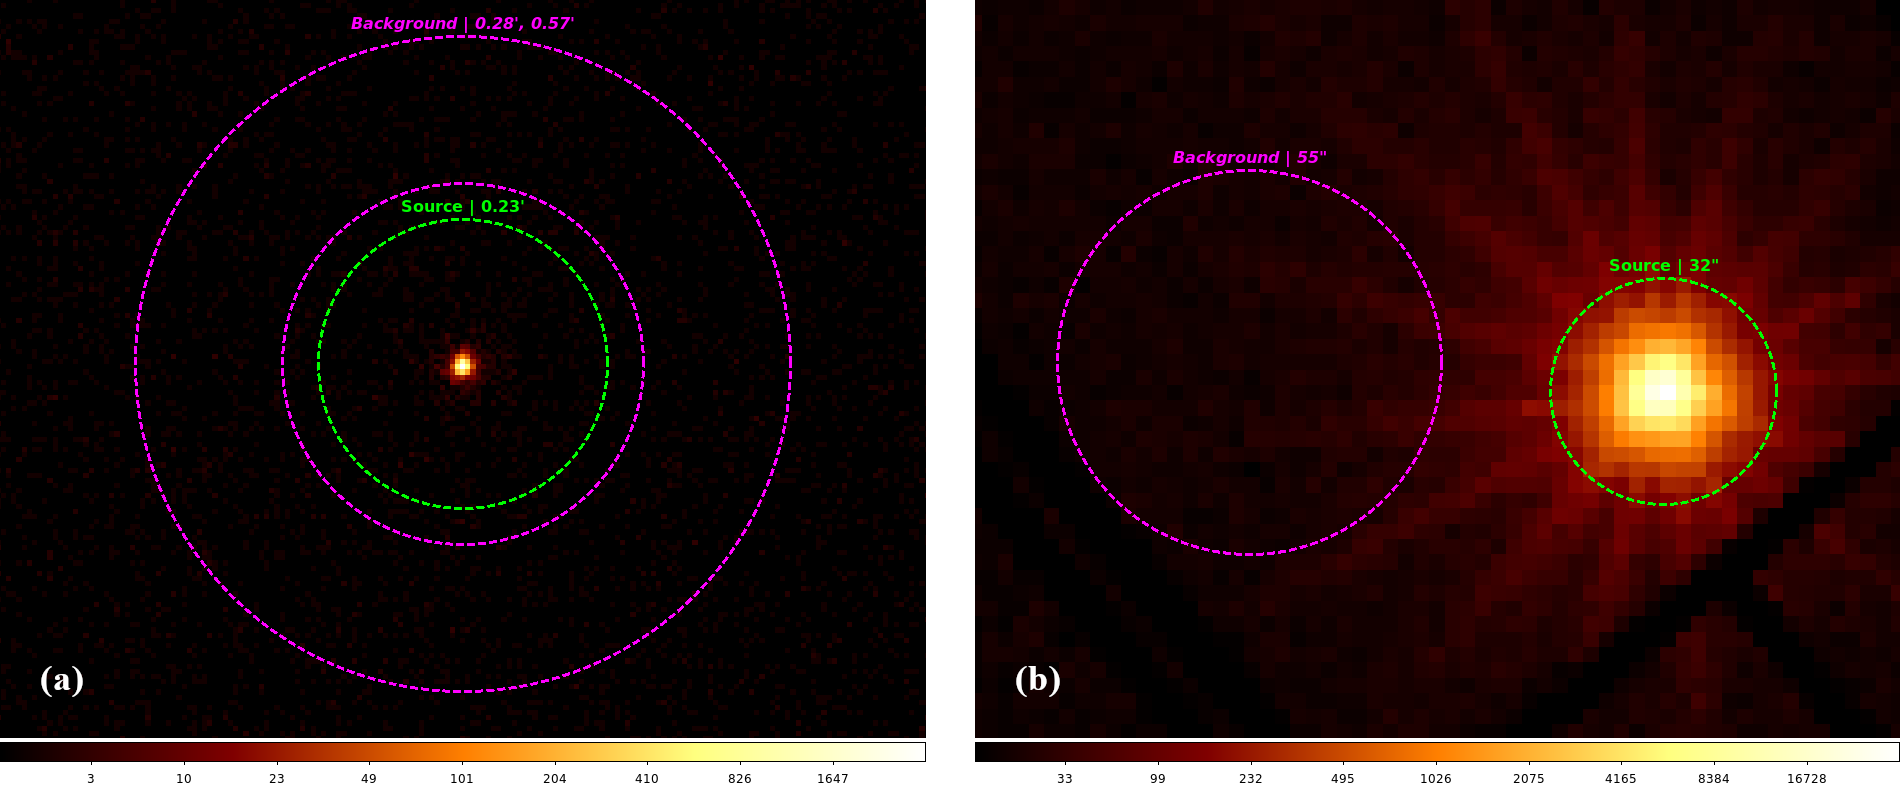
\includegraphics[width=\textwidth]{figures/rx-j0925-7-4758_src-bkg}
	        %\caption{Source and background extraction regions from imaging observation of \source\ with (\textbf{a}) for Chandra }
	        \caption{Extraction regions from imaging observations of \source. (\textbf{a}) Circular region of 0.23' radius for source photons and annular region of 0.28' and 0.57' inner and outer radii with \textit{Chandra} observation, and (\textbf{b}) circular regions of 0.32'' radius for source photons and of 0.55'' radius with \textit{XMM-Newton} observation.}
	        \label{fig:src-bkg}
	    \end{figure*}
	    
%	    \begin{figure*}[!htb]
%        \centering
%        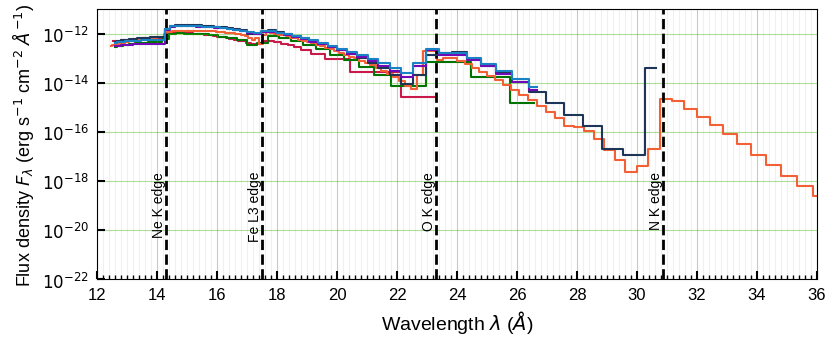
\includegraphics[width=0.8\textwidth]{figures/eufspec/mr-vel-uf-ang_abs-edge.png}
%        \caption{Unfolded spectra with overlaid elemental absorption edges}
%        \label{fig:all-uf:abs-edges}
%    \end{figure*}
    
    \subsection{Chandra ACIS data reduction}
    	\source\ was observed during 14 November 2000 for a duration of $\sim 57$ ks using the High-Energy Transmission Grating Spectrometer (HETGS) on-board NASA's \textit{Chandra} X-ray Observatory. %\cite{beardaChandra2002AA}. 
    	The photons were detected with the ACIS-S CCD array at the focal plane. The data analysis was performed in the energy range 0.4--1.0 keV, with 0.4 keV being the lower limit of the HETGS+ACIS-S spectrometer combination. The extraction of the spectrum and response files was performed using \href{https://cxc.cfa.harvard.edu/ciao/}{CIAO} version 4.10 and the \textit{Chandra} calibration database \href{https://cxc.cfa.harvard.edu/caldb/}{CALDB} version 4.7.7.
%    	\begin{figure}[!htb]
%	        \centering
%	        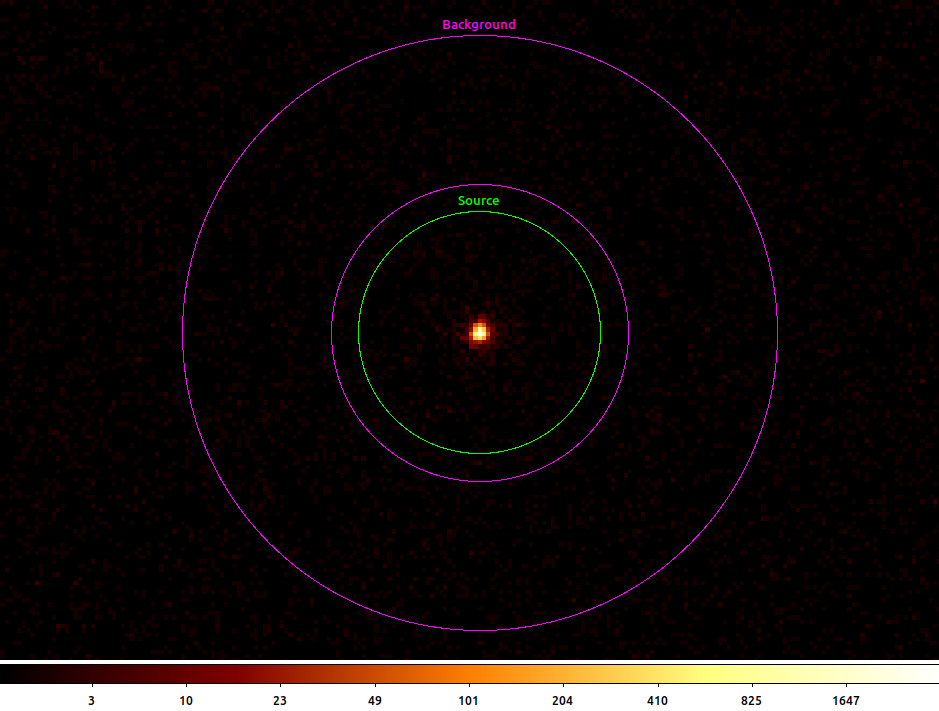
\includegraphics[width=0.45\textwidth]{figures/rx-j0925-7-4758_644_src-bkg.png}
%	        \caption{Source and background extraction regions for the Chandra observation of \source}
%	        \label{fig:src-bkg:acis}
%	    \end{figure}
    	
    	All the science data files were downloaded from HEASARC. \href{https://sites.google.com/cfa.harvard.edu/saoimageds9}{DS9} was used to identify the source and background regions as being a circular region of radius 0.23' and an annular region of radii 0.28' and 0.57' respectively. These photon extraction regions for both source and background are illustrated in figure \ref{fig:src-bkg}(a). The source and background spectra were extracted as FITS files using the task %\texttt{specextract}$^{13}$
    	\href{https://cxc.cfa.harvard.edu/ciao/ahelp/specextract.html}{\texttt{specextract}} using standard parameters as per the %data analysis thread for point-like sources$^{14}$
    	\href{https://cxc.cfa.harvard.edu/ciao/threads/pointlike/}{data analysis thread for point-like sources}. %The resulting source and background extraction regions are presented in figure \ref{fig:src-bkg}(a).
    	
    	The relevant RMF and ARF were generated using the %\texttt{mkacisrmf}$^{15}$
    	\href{https://cxc.cfa.harvard.edu/ciao/ahelp/mkacisrmf.html}{\texttt{mkacisrmf}} and %\texttt{mkarf}$^{16}$
    	\href{https://cxc.cfa.harvard.edu/ciao/ahelp/mkarf.html}{\texttt{mkarf}} tasks respectively. The spectrum set was grouped and binned to have a minimum of 10 counts/bin using the task \texttt{grphha} for subsequent analysis using XSPEC.
    	
    \subsection{XMM-Newton EPIC-pn data reduction}
    	The SSS \source\ was observed by all the instruments, viz. EPIC-MOS 1, EPIC-MOS 2, EPIC-pn and RGS, on-board ESA's \textit{XMM-Newton} observatory for $\sim 61$ ks on 16 December 2000. Whereas, we had retrieved data from all the instruments, in the current work we decided to use only the EPIC-pn data. The reason for this being two-fold:
    	\begin{enumerate}[a)]
    		\item The spectral region of interest is of the lowest energies detectable by EPIC, and the pn detector has a comparatively higher sensitivity than the MOS detectors at lower energies \cite{stecchini2023revisiting,mateos2009statistical}.
    		\item Currently, the high resolution grating spectra (such as those produced by the RGS) yield unacceptable fits to atmosphere models of SSS. Also, no NLTE atmosphere model has yet been able to reproduce all the details in such grating spectra \cite{ness2020complications}.
    	\end{enumerate}
    	As per recommendations by the %\textit{XMM-Newton} SOC$^6$
    	\href{https://xmmweb.esac.esa.int/docs/documents/CAL-TN-0018.pdf}{\textit{XMM-Newton} SOC}, the data analysis was restricted to energies above 0.2 keV. The data reduction procedures were performed using the \textit{XMM-Newton} Science Analysis System (SAS) version 21.0.0.
    
    	The Observation Data Files (ODF) were downloaded from HEASARC. In order to prepare the data for processing, we included the instrumental and calibration information by creating a Calibration Index File (CIF), which was up-to-date with the %current calibration files (CCF)$^7$
    	\href{https://www.cosmos.esa.int/web/xmm-newton/current-calibration-files}{current calibration files (CCF)}, and an extended ODF summary file. These were done by running the SAS tasks \href{https://heasarc.gsfc.nasa.gov/docs/xmm/sas/USG/cifbuild.html}{\texttt{cifbuild}} and \href{https://heasarc.gsfc.nasa.gov/docs/xmm/sas/USG/odfingest.html}{\texttt{odfingest}} respectively. The ODFs were then reprocessed to generate the calibrated event files using the \href{https://heasarc.gsfc.nasa.gov/docs/xmm/sas/help/epproc/index.html}{\texttt{epproc}}, using the default parameters. The event file for EPIC-pn was filtered using the canned screening set of flags, and by setting \texttt{PATTERN==0} to select only single-pixel events in order to maximise energy calibration and resolution. The procedure described by Jethwa et al. (2015) \cite{jethwa2015pile} was used to check and find that the spectral distortion and flux loss both $<0.01\%$, which implied that the pile-up effects could be neglected.
%	    \begin{figure}[!htb]
%	        \centering
%	        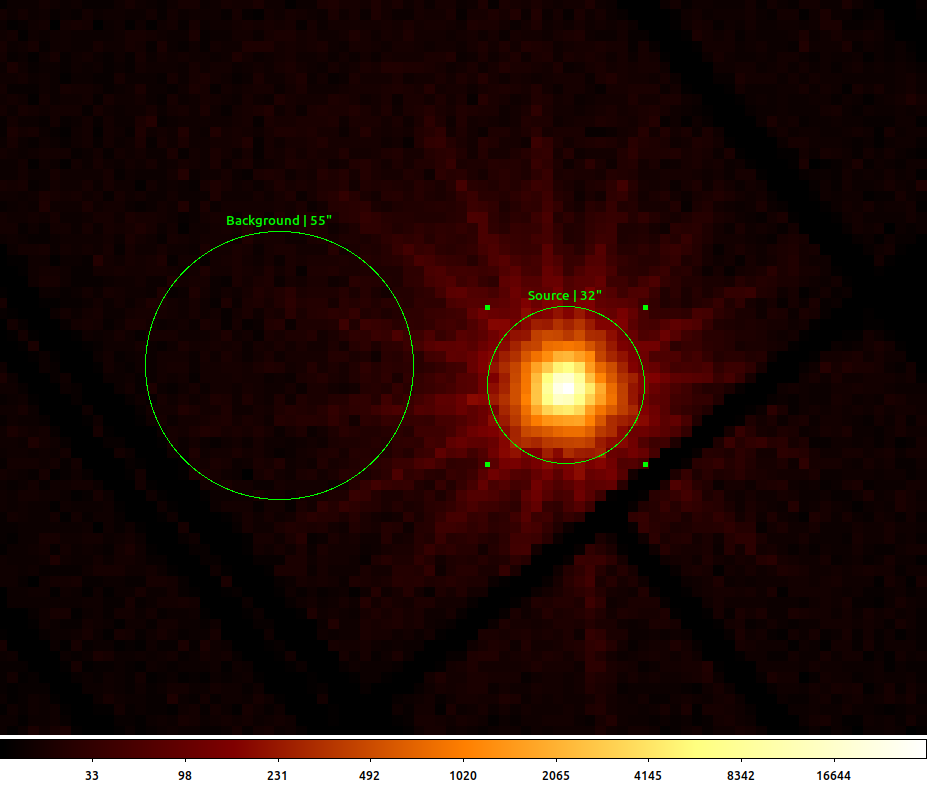
\includegraphics[width=0.45\textwidth]{figures/rx-j0925-7-4758_0111150101_src-bkg.png}
%	        \caption{Source and background extraction regions for the XMM-Newton observation of \source}
%	        \label{fig:src-bkg:pn}
%	    \end{figure}
    
    	The source photons were identified using DS9 and extracted from a circular region having a radius of 30" which is centred at the \source\ centroid position, encompassing about 85-90\% of %\textit{XMM-Newton}'s telescope's on-axis PSF$^8$
    	\href{https://xmm-tools.cosmos.esa.int/external/xmm_user_support/documentation/uhb/onaxisxraypsf.html}{\textit{XMM-Newton}'s telescope's on-axis PSF}. For the background photons, first the SAS task \href{https://heasarc.gsfc.nasa.gov/docs/xmm/sas/help/ebkgreg/ebkgreg.html}{\texttt{ebkgreg}} was executed to obtain an optimum circular background extraction region of radius $\sim$55". The resulting source and background extraction regions are displayed in figure \ref{fig:src-bkg}(b). The RMF and ARF were generated using the standard SAS tasks \href{http://xmm-tools.cosmos.esa.int/external/sas/current/doc/rmfgen/index.html}{\texttt{rmfgen}} and \href{http://xmm-tools.cosmos.esa.int/external/sas/current/doc/arfgen/index.html}{\texttt{arfgen}}. The spectrum was finally binned to have a minimum of 10 counts/bin using the task \texttt{grphha} in order to make it ready for analysis using XSPEC.
    
    \subsection{NICER XTI data reduction}
    	\source\ was observed by the XTI instrument of the \textit{NICER} observatory aboard the \textit{International Space Station} for a total duration of $\sim 21$ ks on three occasions during 18--19 May 2019. All data reduction commands for the science data were performed using \textit{NICER}-specific tasks are made available with the latest versions of %HEASoft$^{17}$
    	HEASoft.
    	
    	The XTI observation dataset and auxiliary files were downloaded from HEASARC. In order to prepare the data for processing, we set up the %remote access of the HEASARC CALDB
    	\href{https://heasarc.gsfc.nasa.gov/docs/heasarc/caldb/caldb_remote_access.html}{remote access of the HEASARC CALDB} by following the recommended %procedure$^{18}$
    	procedure. The cleaned event files were extracted using the %\texttt{nicerl2}$^{19}$
    	\href{https://heasarc.gsfc.nasa.gov/lheasoft/ftools/headas/nicerl2.html}{\texttt{nicerl2}} command. They were then loaded into XSELECT. This produces the source and background spectrum files in FITS format. The ARF and RMF were generated with the extracted source spectrum files using the %\texttt{nicerarf}$^{20}$
    	\href{https://heasarc.gsfc.nasa.gov/lheasoft/ftools/headas/nicerarf.html}{\texttt{nicerarf}} and the %\texttt{nicerrmf}$^{21}$
    	\href{https://heasarc.gsfc.nasa.gov/lheasoft/ftools/headas/nicerrmf.html}{\texttt{nicerrmf}} commands respectively. The spectrum set was finally grouped and binned to a minimum of 10 counts/bin using \texttt{grphha} and made ready for analysis using XSPEC.
    \section{Results}
    Will contain a presentation of the various spectral fitting results in figures and tables.

    To perform fitting of NICER data \cite{orio2022nicer}

    \subsection{Observed count rates}
    In figure \ref{fig:all-counts}, we present a comparison of count rates derived from the multi-satellite observations listed in table \ref{tab:obs-journal}. Figure \ref{fig:all-counts:unnorm} serves to illustrate the variability of flux across different observation epochs, with count rates plotted on a logarithmic scale. This visualization provides insights into the temporal evolution of X-ray emission from \source.

    \begin{figure*}[!htb]
        \centering
        \begin{subfigure}[b]{0.45\textwidth}
            \centering
            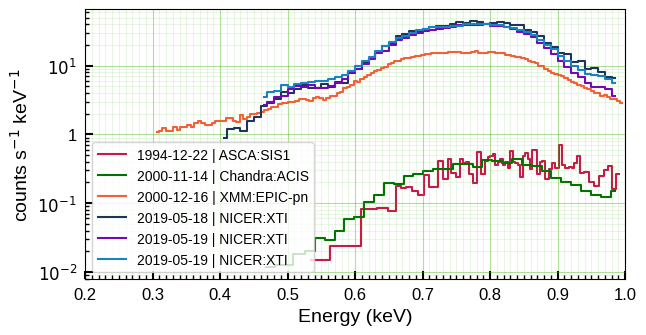
\includegraphics[width=\textwidth]{figures/ldata/mr-vel-counts_all-obs.png}
            \caption{Comparison of flux from all observations from their count rates plotted to scale}
            \label{fig:all-counts:unnorm}
        \end{subfigure}
        \hfill
        \begin{subfigure}[b]{0.45\textwidth}
            \centering
            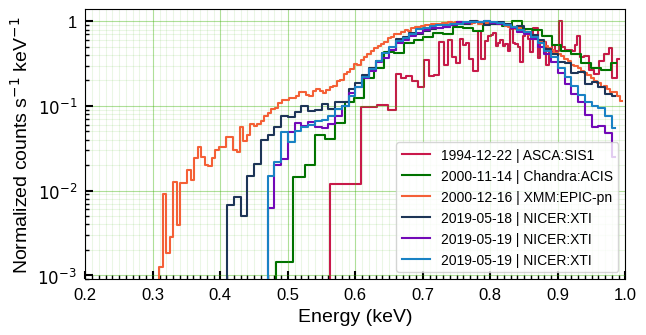
\includegraphics[width=\textwidth]{figures/ldata/mr-vel-normcounts_all-obs.png}
            \caption{Normalized count rates from all observations show varying responses to supersoft X-rays}
            \label{fig:all-counts:norm}
        \end{subfigure}
        \caption{Count rates from observational dataset}
        \label{fig:all-counts}
    \end{figure*}
    
    Concurrently, in figure \ref{fig:all-counts:norm}, the count rates are normalized to the range of 0 to 1 using \textit{min-max normalization}. This visualization accentuates the relative sensitivity of more recent observations to supersoft X-ray photons emitted by MR Vel. The sub-plot shows that in recent observations the supersoft X-ray features are discernibly enhanced. This might be suggestive of improved observational capabilities or heightened sensitivity to the emitted X-ray flux.
    
    Together, these visualizations offer a nuanced understanding of the flux variability and observational sensitivity trends exhibited by MR Vel across different observation epochs, contributing to the broader understanding of its X-ray emission characteristics.
    
    \subsection{NLTE continuum model}
    In table \ref{tab:res-fitting}, we present the luminosity, effective temperature and column density for \source\ which are derived after performing the fitting to the NLTE continuum model described in section \ref{sec:reduction-analysis}. We also present the model fit statistics, namely the reduced $\chi^2$ values for each fit. It can be noticed that the same continuum model has been able to provide a good fit to all of the observations in our chosen dataset.
    \begin{table*}[!htb]
    	\centering
    	\caption{Parameters of \source\ derived from continuum NLTE model from multi-observatory observations.}
    	\label{tab:res-fitting}
    	\begin{tabular}{ccccccc}
			\hline
			{\textbf{Observatory}} & {\textbf{Obs. ID}} & {$\boldsymbol{L_*}$} & {\textbf{$\boldsymbol{T_\text{eff}}$ (kK)}} & {\textbf{$\boldsymbol{n_H}$ (cm$^{-2}$)}} & {$\boldsymbol{\chi^2}$/\textbf{d.o.f}} & {$\boldsymbol{\chi^2_\text{reduced}}$} \\
			\hline
			{ASCA} & {43036000} & {TBC} & {$100.6_{70.1}^{140.9}$} & {$0.75_{0.00}^{2.45}$} & {75.8/63} & {1.20} \\
			{Chandra} & {644} & {TBC} & {$84.0_{70.6}^{92.7}$} & {$1.77_{1.52}^{1.96}$} & {41.0/30} & {1.37} \\
			{XMM-Newton} & {0111150101} & {TBC} & {$80.0_{70.7}^{80.5}$} & {$1.81_{1.67}^{1.93}$} & {176.5/132} & {1.34} \\
			{NICER} & {2611020101} & {TBC} & {$90.8_{80.1}^{109.9}$} & {$1.33_{0.92}^{1.73}$} & {70.9/51} & {1.39} \\
			{NICER} & {2611020102} & {TBC} & {TBC} & {TBC} & {55.2/45} & {1.23} \\
			{NICER} & {2611020103} & {TBC} & {$113.5_{103.9}^{122.4}$} & {$0.74_{0.57}^{0.97}$} & {68.2/45} & {1.52} \\
			\hline
		\end{tabular}
	\end{table*}
    
    \subsection{Unfolded spectra}
    In figure \ref{fig:all-uf}, the unfolded spectrum, which is obtained after fitting the data to the best-fit model, is displayed. Observations in panels \ref{fig:all-uf:12-24} and \ref{fig:all-uf:24-36} reveal features which are indicative of the presence of elemental absorption edges.
    
    \begin{figure*}[!bht]
        \centering
        \begin{subfigure}[b]{0.45\textwidth}
            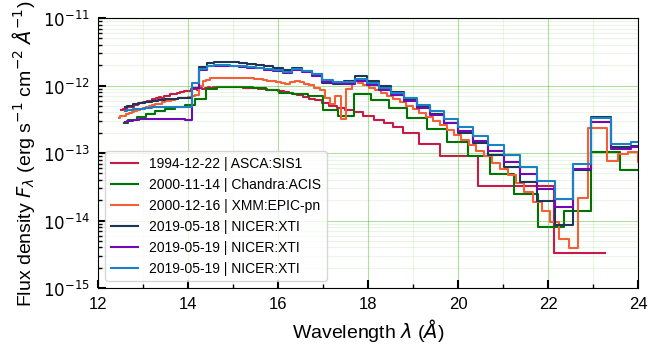
\includegraphics[width=\textwidth]{figures/eufspec/mr-vel-uf_all-obs_12-24.png}
            \caption{Unfolded spectra after model fitting in the range 12 \AA - 24 \AA}
            \label{fig:all-uf:12-24}
        \end{subfigure}
        \hfill
        \begin{subfigure}[b]{0.45\textwidth}
            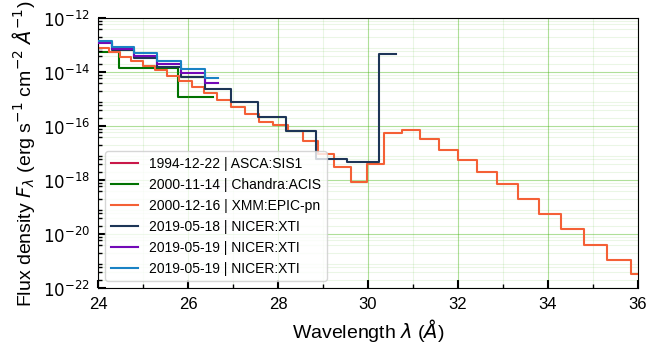
\includegraphics[width=\textwidth]{figures/eufspec/mr-vel-uf_all-obs_24-36.png}
            \caption{Unfolded spectra after model fitting in the range 24 \AA - 36 \AA}
            \label{fig:all-uf:24-36}
        \end{subfigure}
        \caption{Unfolded spectra after model fitting}
        \label{fig:all-uf}
    \end{figure*}

    \subsection{Presence of elemental absorption edges}
    Four elemental absorption edges were detected upon the inspection of the unfolded spectra obtained from the best fitting model on all the observations. These absorption edges, belonging to N, O, Ne and Fe, are overlaid on the unfolded spectra and displayed in figure \ref{fig:all-uf:abs-edges}.
    \begin{figure*}[!htb]
        \centering
        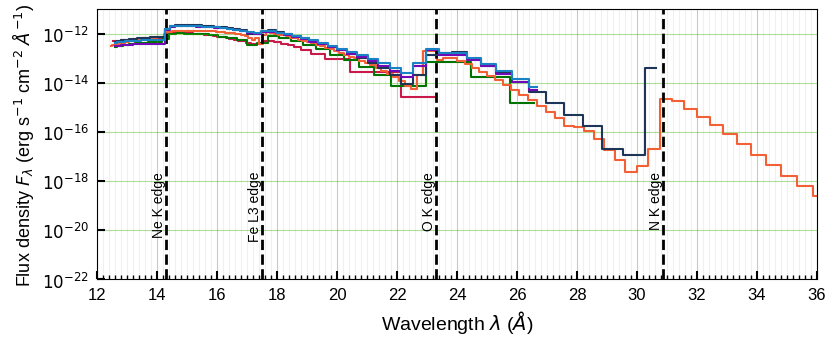
\includegraphics[width=0.8\textwidth]{figures/eufspec/mr-vel-uf-ang_abs-edge.png}
        \caption{Unfolded spectra with overlaid elemental absorption edges}
        \label{fig:all-uf:abs-edges}
    \end{figure*}
    
    \begin{table*}[!htb]
    	\centering
    	\caption{Absorption depth $D$ of \source\ derived from identified absorption edges of Ne, Fe, O and N.}
    	\label{tab:abs-depth}
		\begin{tabular}{cccccc}
			\hline
			\multirow{3}{*}{\textbf{Observatory}} & \multirow{3}{*}{\textbf{Obs. ID}} & \multicolumn{4}{c}{\textbf{Absorption Depth $\boldsymbol{D}$}} \\ \cline{3-6} & & \textbf{Ne $\boldsymbol{K}$ edge} & \textbf{Fe $\boldsymbol{L_3}$ edge} & \textbf{O $\boldsymbol{K}$ edge} & \textbf{N $\boldsymbol{K}$ edge} \\ \cline{3-6} & & \textbf{14.302 \AA} & \textbf{17.509 \AA} & \textbf{23.305 \AA} & \textbf{30.873 \AA} \\
			\hline
			{ASCA} & {43036000} & {0.504} & {0.664} & {0.943} & {1.780} \\
			{Chandra} & {644} & {0.356} & {0.644} & {1.654} & {5.076} \\
			{XMM-Newton} & {0111150101} & {0.027} & {0.160} & {0.184} & {4.998} \\
			{NICER} & {2611020101} & {0.652} & {0.080} & {1.771} & {0.010} \\
			{NICER} & {2611020102} & {1.524} & {0.208} & {0.476} & {1.755} \\
			{NICER} & {2611020103} & {TBC} & {TBC} & {TBC} & {TBC} \\
			\hline
		\end{tabular}
	\end{table*}

    Because the best-fitted spectrum obtained from the EPIC-pn instrument of XMM-Newton spans the widest range of wavelengths, known absorption edges \cite{bearden1967reevaluation,juett2006high} were identified in the vicinity of the absorption edges in figure \ref{fig:all-uf:abs-edges}. These are reported in table \ref{tab:abs-depth}. Then they were overlaid on the unfolded spectrum obtained from the EPIC-pn observation. The four absorption edges that could be identified are the K edges of N, O and Ne and the L$_3$ edge of Fe at 30.873 \AA, 23.305 \AA, 14.302 \AA and 17.509 \AA respectively, as displayed in the sub-plots of figure \ref{fig:pn-uf:abs-edges}.

    \begin{figure*}[!bht]
        \centering
        \begin{subfigure}[b]{0.45\textwidth}
            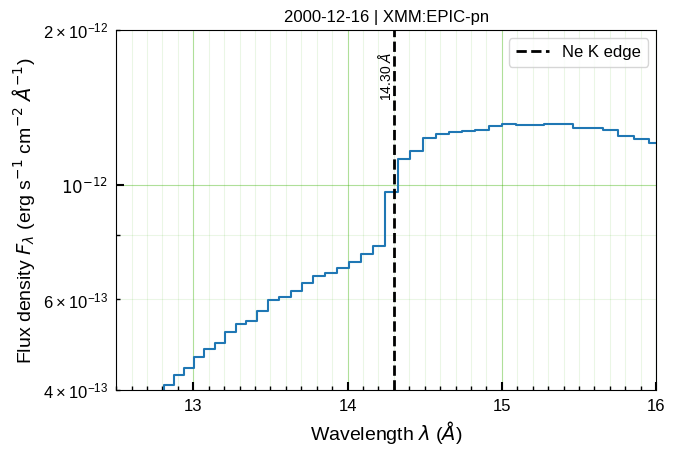
\includegraphics[width=\textwidth]{figures/eufspec/mr-vel-XMM-EPIC-pn-uf-Ne-edges.png}
            \caption{Ne K absorption edge at 14.302 \AA}
            \label{fig:pn-uf:Ne-edges}
        \end{subfigure}
        \hfill
        \begin{subfigure}[b]{0.45\textwidth}
            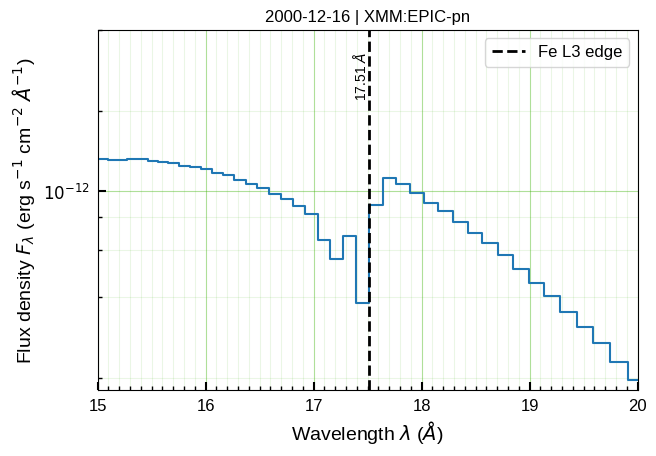
\includegraphics[width=\textwidth]{figures/eufspec/mr-vel-XMM-EPIC-pn-uf-Fe-edges.png}
            \caption{Fe L$_3$ absorption edge at 17.509 \AA}
            \label{fig:pn-uf:Fe-edges}
        \end{subfigure}
        \begin{subfigure}[b]{0.45\textwidth}
            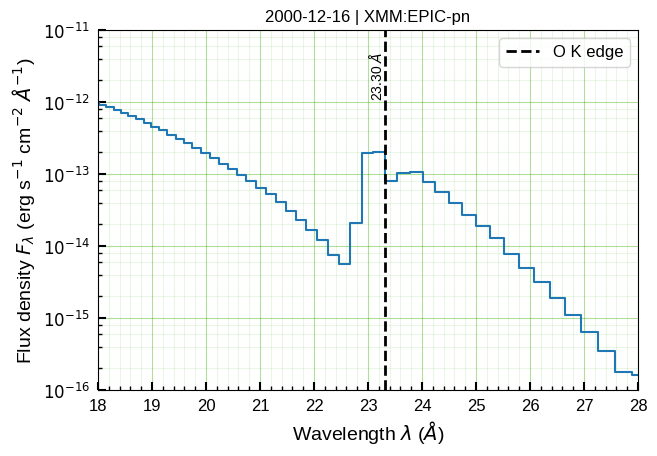
\includegraphics[width=\textwidth]{figures/eufspec/mr-vel-XMM-EPIC-pn-uf-O-edges.png}
            \caption{O K absorption edge at 23.305 \AA}
            \label{fig:pn-uf:O-edges}
        \end{subfigure}
        \hfill
        \begin{subfigure}[b]{0.45\textwidth}
            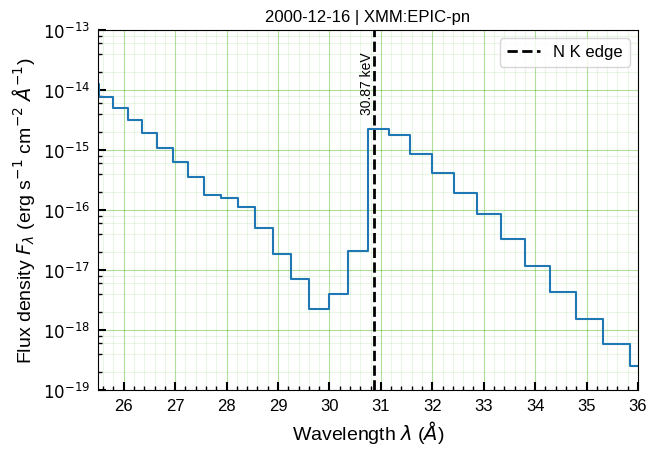
\includegraphics[width=\textwidth]{figures/eufspec/mr-vel-XMM-EPIC-pn-uf-N-edges.png}
            \caption{N K absorption edge at 30.873 \AA}
            \label{fig:pn-uf:N-edges}
        \end{subfigure}
        \caption{Absorption edges for N, O, Ne and Fe overlaid on the unfolded spectrum for EPIC-pn observation}
        \label{fig:pn-uf:abs-edges}
    \end{figure*}

    \section{Discussion and Conclusions}
	
	\begin{itemize}
		\item To include a detailed description of the physics behind the best fit model
		\item To refer to the original publications containing the XSPEC model components where the physics is described
		\begin{itemize}
			\item For \texttt{TBabs}: Wilms et al. \url{https://iopscience.iop.org/article/10.1086/317016/pdf}
			
			Now \texttt{phabs}
			\item For \texttt{ismabs}: Gatuzz et al. \url{https://iopscience.iop.org/article/10.1088/0004-637X/800/1/29/pdf}
			\item For \texttt{edge}: \url{https://heasarc.gsfc.nasa.gov/xanadu/xspec/manual/node247.html}
			\item For \texttt{rauch}: \url{http://astro.uni-tuebingen.de/~rauch/TMAF/TMAF.html}
		\end{itemize}
	\end{itemize}
	An inspection of the distribution of the residual suggests an approximately normal distribution, which can be observed in the best-fit models for all the observations, further supporting the validity of the model fit with values of $1<\chi^2_\text{red}<2$. Such a distribution of the residuals is displayed in figure \ref{fig:pn:resid-hist} for the observations of the EPIC-pn data.
	
	\begin{figure*}[!htb]
        \centering
        \begin{subfigure}[b]{0.51\textwidth}
            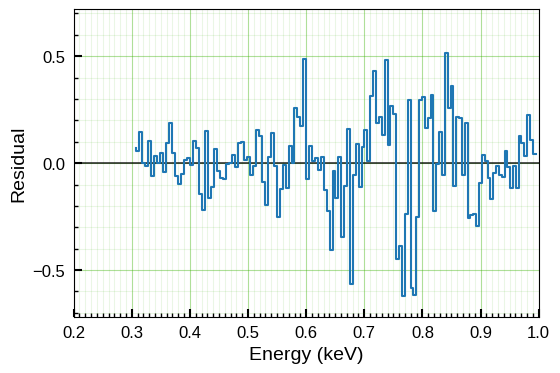
\includegraphics[width=\textwidth]{figures/resid/mr-vel-0111150101-pn_resid.png}
            \caption{Residuals between data and best-fit model for EPIC-pn observations}
            \label{fig:pn:resid}
        \end{subfigure}
        \hfill
        \begin{subfigure}[b]{0.39\textwidth}
            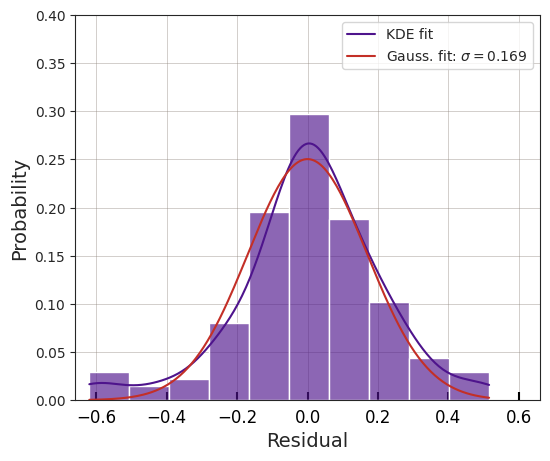
\includegraphics[width=\textwidth]{figures/resid/mr-vel-0111150101-pn_resid-hist.png}
	        \caption{Distribution of residuals from the best-fit model to EPIC-pn observations, along with the KDE function and fitted Gaussian}
	        \label{fig:pn:resid-hist}
        \end{subfigure}
        \caption{Residual statistics from best-fit model to all observations}
        \label{fig:all-obs:resid-stats}
    \end{figure*}
    
    As it can be seen in figure \ref{fig:pn:resid-hist}, the kernel density estimate (KDE) function of the distribution closely approximates a normal distribution centred about zero (zero indicating a perfect fit) and with a standard deviation of 0.169, thereby indicating that the observed count rate data can be considered to be random fluctuations which are normally distributed about the best-fit model.
    
    \begin{figure}[!htb]
    	\centering
    	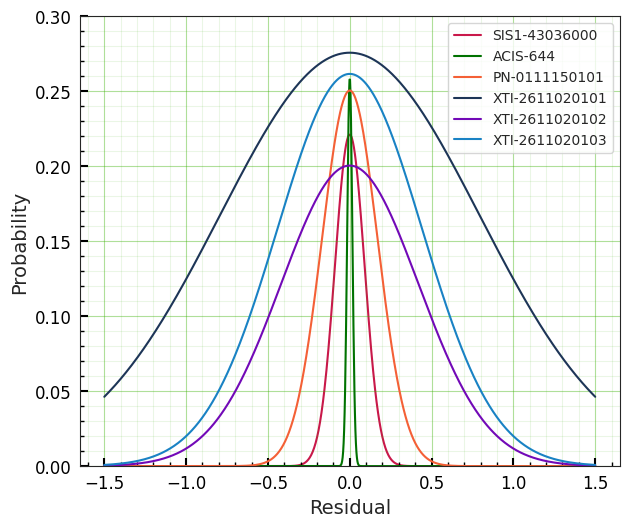
\includegraphics[width=0.45\textwidth]{figures/resid/mr-vel-resid-gaussfit_all-obs.png}
    	\caption{Gaussian approximations of the KDE functions for residual distributions of all observations}
    	\label{fig:all-obs:resid-gaussfit}
    \end{figure}
    
    In figure \ref{fig:all-obs:resid-gaussfit}, we find the Gaussian distribution fitted to all the observations. This figure shows that the quality of the fit is the best for the earlier Chandra, XMM-Newton and ASCA observations. For the recent NICER observations, the residuals show a wider spread spread about the perfect fit.
    
    %% Appendices    
    \appendix
        \section{An appendix section}
    Text goes here.
    \begin{equation}
    x=a+b+c
    \end{equation}

        \section{Another appendix section}
    Text goes here.
    \begin{equation}
    y^2=ax+b+c
    \end{equation}

    
    %% Acknowledgements
    \section*{Acknowledgement}
%    To acknowledge the contributions from the following:
%    \begin{itemize}
%        \item Paulo Stecchini
%        \item Jan-Uwe Ness
%        \item Santosh Jagade, IUCAA
%        \item ASSC
%    \end{itemize}
	We extend our heartfelt gratitude to Paulo E. F. Stecchini from Instituto de Astronomia, S\~{a}o Paulo, Brazil, for his patient responses to our inquiries regarding spectral analysis. His expertise and guidance were indispensable in aiding our comprehension of the nuances of data and the spectral fitting procedure. We also extend our appreciation to Jan-Uwe Ness from the European Space Agency, Madrid, Spain, for illuminating the underlying astrophysical principles involved in data analysis, thereby enriching our understanding. Additionally, we acknowledge Santosh Jagade, Scientific Officer at the Computing Facility, IUCAA, Pune, for his consistent availability and valuable technical assistance throughout our analysis. Finally, we express gratitude to the Astrosat Science Support Cell (ASSC), IUCAA, Pune, for granting us remote access to their high-performance computing facility, significantly facilitating our data processing and analysis.    
    
    %%use \balance somewhere in the left column of the last page to balance the two columns in the end page
    
    %% References
    %\bibliography{myref}

% -------------- Journal abbreviations --------------
\newcommand{\Nat}{Nature}
\newcommand{\AnA}{Astron. Astrophys.}
\newcommand{\AnASS}{Astron. Astrophys. Suppl. Series}
\newcommand{\ARAA}{Ann. Rev. Astron. Astrophys.}
\newcommand{\ApJ}{Astrophys. J.}
\newcommand{\PASP}{Publ. Astron. Soc. Pacific}
\newcommand{\NA}{New Astron.}
\newcommand{\ANAN}{Astron. Nachr.: Astron. Notes}
\newcommand{\MNRAS}{Mon. Not. R. Astron. Soc.}
\newcommand{\ASR}{Adv. Space Res.}
\newcommand{\RMP}{Rev. Mod. Phys.}
\newcommand{\Pram}{Pramana}
\newcommand{\SAM}{Stellar Atmos. Modeling}
\newcommand{\JCAM}{J. Comput. Appl. Math.}
\newcommand{\AJET}{ADBU J. Eng. Technol.}
\newcommand{\ARX}{arXiv preprint}

% --------------- Bibliography entries ---------------
\begin{thebibliography}{100}
	\bibitem{long81}
	K S Long, D J Helfand and D A Grabelsky, \textit{\ApJ}, \textbf{248}, 925 (1981)
	
	\bibitem{trumper1991x}
	J Tr{\"u}mper, G Hasinger, B Aschenbach, H Braeuninger, U G Briel, W Burkert, H Fink, E Pfeffermann, W Pietsch, P Predehl, J H M M Schmitt, W Voges, U Zimmermann and K Beuermann, \textit{\Nat}, \textbf{349}, 579 (1991)
	
	\bibitem{greiner1991rosat}
	J Greiner, G Hasinger and P Kahabka, \textit{\AnA}, \textbf{246}, L17 (1991)
	
	\bibitem{kahabka97}
	P Kahabka and E P J van den Heuvel, \textit{\ARAA}, \textbf{35}, 342 (1997)
	
	\bibitem{kahabka06}
	P Kahabka and E P J van den Heuvel, in \textit{Compact Stellar X-Ray Sources} edited by W H G Lewin and M van der Klis (Cambridge University Press, Cambridge, 2006), Vol. \textbf{1}, p. 461

	\bibitem{kahabkatrumper1996}
	P Kahabka and J Tr{\"u}mper, in \textit{Compact Stars in Binaries} edited by J van Paradijs, E P J van den Heuvel and E Kuulkers (Cambridge University Press, Cambridge, 1996), Vol. \textbf{165}, p. 425

	\bibitem{steinerdiaz1998}
	J E Steiner and M P Diaz, \textit{\PASP}, \textbf{110}, 276 (1998)

	\bibitem{greiner2000}
	J Greiner, \textit{\NA}, \textbf{5}, 137 (2000)

	\bibitem{pietsch2003deep}
	W Pietsch, M Ehle, F Haberl, Z Misanovic and G Trinchieri, \textit{\ANAN}, \textbf{324}, 85 (2003)

	\bibitem{di2003luminous}
	R di Stefano and A K H Kong, \textit{\ApJ}, \textbf{592}, 884 (2003)

	\bibitem{orio2010census}
	M Orio, T Nelson, A Bianchini, F di Mille and D Harbeck, \textit{\ApJ}, \textbf{717}, 739 (2010)

	\bibitem{henze2010recent}
	M Henze, W Pietsch, F Haberl, G Sala, M Hernanz, D Hatzidimitriou, A Rau, D H Hartmann, J Greiner, M Orio, H Stiele and M J Freyberg, \textit{\ANAN}, \textbf{331}, 193 (2010)

	\bibitem{sturm2012new}
	R Sturm, F Haberl, W Pietsch, M J Coe, S Mereghetti, N la Palombara,
R A Owen and A Udalski, \textit{\AnA}, \textbf{537}, A76 (2012)

	\bibitem{galiullin2021populations}
	I Galiullin and M Gilfanov, \textit{\AnA}, \textbf{646}, A85 (2021)
	
	\bibitem{van1992accreting}
	E P J van den Heuvel, D Bhattacharya, K Nomoto and S A Rappaport, \textit{\AnA}, \textbf{262}, 97 (1992)
	
	\bibitem{kylafis93}
	N D Kylafis and E M Xilouris, \textit{\AnA}, \textbf{278}, L43 (1993)

	\bibitem{vandenHeuvel92}
	E P J van den Heuvel, D Bhattacharya, K Nomoto and S A Rappaport, \textit{\AnA}, \textbf{262}, 97 (1992)
	
	\bibitem{paczynski78}
	B Paczy{\'n}ski and A N Zytkow, \textit{\ApJ}, \textbf{222}, 604 (1978)
	
	\bibitem{prialnik78}
	D Prialnik, M M Shara and G Shaviv, \textit{\AnA}, \textbf{62}, 339 (1978)

	\bibitem{sion79}
	E M Sion, M J Acierno and S Tomczyk, \textit{\ApJ}, \textbf{230}, 832 (1979)

	\bibitem{sienkiewicz80}
	R Sienkiewicz, \textit{\AnA}, \textbf{85}, 295 (1980)
	
	\bibitem{nomoto82}
	K Nomoto, \textit{\ApJ}, \textbf{253}, 798 (1982)
	
	\bibitem{fujimoto82a}
	M Y Fujimoto, \textit{\ApJ}, \textbf{257}, 752 (1982)
	
	\bibitem{fujimoto82b}
	M Y Fujimoto, \textit{\ApJ}, \textbf{257}, 767 (1982)
	
	\bibitem{iben82}
	I Iben, \textit{\ApJ}, \textbf{259}, 244 (1982)

	\bibitem{prialnik95}
	D Prialnik and A Kovetz, \textit{\ApJ}, \textbf{445}, 789 (1995)
	
	\bibitem{macdonald83}
	J MacDonald, \textit{\ApJ}, \textbf{267}, 732 (1983)
	
	\bibitem{paczynski80}
	B Paczy{\'n}ski and B Rudak, \textit{\AnA}, \textbf{82}, 349 (1980)
	
	\bibitem{hachisu2001}
	I Hachisu and M Kato, \textit{\ApJ}, \textbf{558}, 323 (2001)
	
	\bibitem{motch1994}
	C Motch, G Hasinger and W Pietsch, \textit{\AnA}, \textbf{284}, 827 (1994)

	\bibitem{hartmann1999constraining}
	H W Hartmann, J Heise, P Kahabka, C Motch and A N Parmar, \textit{\AnA}, \textbf{346}, 125 (1999)
	
	\bibitem{beardaChandra2002AA}
	H Bearda, W Hartmann, K Ebisawa, J Heise, J Kaastra, R van der Meer, F Verbunt and C Motch, \textit{\AnA}, \textbf{385}, 511 (2002)

	\bibitem{motchXmmNewton2002AA}
	C Motch, H Bearda and C Neiner, \textit{\AnA}, \textbf{393}, 913 (2002)

	\bibitem{ebisawaAsca2001ApJ}
	K Ebisawa, K Mukai, T Kotani, K Asai, T Dotani, F Nagase, H W Hartmann, J Heise, P Kahabka and A van Teeseling, \textit{\ApJ}, \textbf{550}, 1007 (2001)

	\bibitem{orioNicer2022ApJ}
	M Orio, K Gendreau, M Giese, G J M Luna, J Magdolen, S Pei, B Sun, E Behar, A Dobrotka, J Mikolajewska, D R Pasham and T E Strohmayer, \textit{\ApJ}, \textbf{932}, 45 (2022)
	
	\bibitem{stecchini2023revisiting}
	P E Stecchini, M P Diaz, F D’Amico and F Jablonski, \textit{\MNRAS}, \textbf{522}, 3472 (2023)
	
	\bibitem{mateos2009statistical}
	S Mateos, R D Saxton, A M Read and S Sembay, \textit{\AnA}, \textbf{496}, 879 (2009)
	
	\bibitem{ness2020complications}
	J Ness, \textit{\ASR}, \textbf{66}, 1202 (2020)
	
	\bibitem{jethwa2015pile}
	P Jethwa, R Saxton, M Guainazzi, P Rodriguez-Pascual and M Stuhlinger, \textit{\AnA}, \textbf{581}, A104 (2015)
	
	\bibitem{bearden1967reevaluation}
	J A Bearden and A F Burr, \textit{\RMP}, \textbf{39}, 125 (1967)
	
	\bibitem{juett2006high}
	A M Juett, N S Schulz, D Chakrabarty and T W Gorczyca, \textit{\ApJ}, \textbf{648}, 1066 (2006)
	
	\bibitem{prodhani2018galactic}
	N Prodhani and M Baruah, \textit{\Pram}, \textbf{90}, 1 (2018)
	
%	\bibitem{hubeny2014theory}
%	I  Hubeny and D Mihalas, in \textit{Theory of Stellar Atmospheres: An Introduction to Astrophysical Non-Equilibrium Quantitative Spectroscopic Analysis} (Princeton University Press, Princeton, 2014), Vol. \textbf{26}

	\bibitem{hubeny2014theory}
	I  Hubeny and D Mihalas, in \textit{Theory of Stellar Atmospheres} (Princeton University Press, Princeton, 2014), Vol. \textbf{26}
	
	\bibitem{hubeny2003accelerated}
	I Hubeny, \textit{\SAM}, \textbf{288}, 17 (2003)
	
	\bibitem{auer1970non}
	L H Auer and D Mihalas., \textit{\ApJ}, \textbf{160}, 233 (1970)
	
	\bibitem{werner1999classical}
	K Werner and S Dreizler, \textit{JCAM}, \textbf{109}, 65 (1999)
	
	\bibitem{rauch2003grid}
	T Rauch, \textit{\AnA}, \textbf{403}, 709 (2003)
	
	\bibitem{rauch2010nlte}
	T Rauch, M Orio, R Gonzales-Riestra, T Nelson, M Still, K Werner and J Wilms, \textit{\ARX}, \textbf{1006.2918}, (2010)
	
	\bibitem{lemke1997extended}
	M Lemke, \textit{\AnASS}, \textbf{122}, 285 (1997)
	
	\bibitem{bhattacharya2020python}
	P Bhattacharya, B M Lyngdoh, J I Nongrum, R Misra and M Baruah, \textit{\AJET}, \textbf{9}, 1 (2020)
	
	\bibitem{ness2013obscuration}
	J Ness, J P Osborne, M Henze, A Dobrotka, J J Drake, V A R M Ribeiro, S Starrfield, E Kuulkers, E Behar, M Hernanz, G Schwarz, K L Page, A P Beardmore and M F Bode, \textit{\AnA}, \textbf{559}, A50 (2013)
\end{thebibliography}



%	\bibitem{citeID}
%	I Lastname, J Lastname and K Lastname, \textit{Journal Abbr.}, \textbf{vol}, firstpage (year)

%	\bibitem{citeID}
%	I Lastname, J Lastname and K Lastname, in \textit{Full Book Name} edited by I Lastname, J Lastname and K Lastname (Publisher, Place, Year), Vol. \textbf{vol}, p. firstpage


\end{document}
